
%(BEGIN_QUESTION)
% Copyright 2010, Tony R. Kuphaldt, released under the Creative Commons Attribution License (v 1.0)
% This means you may do almost anything with this work of mine, so long as you give me proper credit

A newly-constructed H1 Fieldbus segment seems to have a problem.  The host system (an Emerson DeltaV DCS) recognizes the pressure transmitter, but fails to recognize the control valve positioner when it is connected to the segment.  The positioner does not even come up on the Emerson system as a ``decommissioned'' device -- there simply isn't any ackowledgement from the DCS at all that another device exists on the segment.  A diagram of the system appears here:

$$\includegraphics[width=15.5cm]{i00477x01.eps}$$

The first step you take in diagnosing this problem is to measure DC voltage with your voltmeter at the terminals of the valve positioner.  There, you measure a steady 23.1 volts DC.

\vskip 10pt

Identify the likelihood of each specified fault for this circuit.  Consider each fault one at a time (i.e. no coincidental faults), determining whether or not each fault could independently account for {\it all} measurements and symptoms in this circuit.

% No blank lines allowed between lines of an \halign structure!
% I use comments (%) instead, so that TeX doesn't choke.

$$\vbox{\offinterlineskip
\halign{\strut
\vrule \quad\hfil # \ \hfil & 
\vrule \quad\hfil # \ \hfil & 
\vrule \quad\hfil # \ \hfil \vrule \cr
\noalign{\hrule}
%
% First row
{\bf Fault} & {\bf Possible} & {\bf Impossible} \cr
%
\noalign{\hrule}
%
% Another row
Trunk cable 1 failed open &  &  \cr
%
\noalign{\hrule}
%
% Another row
FF transmitter failed open &  &  \cr
%
\noalign{\hrule}
%
% Another row
FF positioner failed open &  &  \cr
%
\noalign{\hrule}
%
% Another row
Transmitter spur cable failed open &  &  \cr
%
\noalign{\hrule}
%
% Another row
Positioner spur cable failed open &  &  \cr
%
\noalign{\hrule}
%
% Another row
Trunk cable 1 failed shorted &  &  \cr
%
\noalign{\hrule}
%
% Another row
FF transmitter failed shorted &  &  \cr
%
\noalign{\hrule}
%
% Another row
Transmitter spur cable failed shorted &  &  \cr
%
\noalign{\hrule}
%
% Another row
Positioner spur cable failed shorted &  &  \cr
%
\noalign{\hrule}
%
% Another row
Terminator failed open &  &  \cr
%
\noalign{\hrule}
} % End of \halign 
}$$ % End of \vbox

Also, identify one fault not included on this list that is capable of independently accounting for all measurements and symptoms.

Finally, identify the {\it next} diagnostic test or measurement you would make on this system.  Explain how the result(s) of this next test or measurement help further identify the location and/or nature of the fault.

\underbar{file i00477}
%(END_QUESTION)





%(BEGIN_ANSWER)

\noindent
{\bf Partial answer:}

% No blank lines allowed between lines of an \halign structure!
% I use comments (%) instead, so that TeX doesn't choke.

$$\vbox{\offinterlineskip
\halign{\strut
\vrule \quad\hfil # \ \hfil & 
\vrule \quad\hfil # \ \hfil & 
\vrule \quad\hfil # \ \hfil \vrule \cr
\noalign{\hrule}
%
% First row
{\bf Fault} & {\bf Possible} & {\bf Impossible} \cr
%
\noalign{\hrule}
%
% Another row
Trunk cable 1 failed open &  &  \cr
%
\noalign{\hrule}
%
% Another row
FF transmitter failed open &  & $\surd$ \cr
%
\noalign{\hrule}
%
% Another row
FF positioner failed open & $\surd$ &  \cr
%
\noalign{\hrule}
%
% Another row
Transmitter spur cable failed open &  &  \cr
%
\noalign{\hrule}
%
% Another row
Positioner spur cable failed open &  &  \cr
%
\noalign{\hrule}
%
% Another row
Trunk cable 1 failed shorted &  &  \cr
%
\noalign{\hrule}
%
% Another row
FF transmitter failed shorted &  & $\surd$ \cr
%
\noalign{\hrule}
%
% Another row
Transmitter spur cable failed shorted &  &  \cr
%
\noalign{\hrule}
%
% Another row
Positioner spur cable failed shorted &  & $\surd$ \cr
%
\noalign{\hrule}
%
% Another row
Terminator failed open &  &  \cr
%
\noalign{\hrule}
} % End of \halign 
}$$ % End of \vbox


%(END_ANSWER)





%(BEGIN_NOTES)

% No blank lines allowed between lines of an \halign structure!
% I use comments (%) instead, so that TeX doesn't choke.

$$\vbox{\offinterlineskip
\halign{\strut
\vrule \quad\hfil # \ \hfil & 
\vrule \quad\hfil # \ \hfil & 
\vrule \quad\hfil # \ \hfil \vrule \cr
\noalign{\hrule}
%
% First row
{\bf Fault} & {\bf Possible} & {\bf Impossible} \cr
%
\noalign{\hrule}
%
% Another row
Trunk cable 1 failed open &  & $\surd$ \cr
%
\noalign{\hrule}
%
% Another row
FF transmitter failed open &  & $\surd$ \cr
%
\noalign{\hrule}
%
% Another row
FF positioner failed open & $\surd$ &  \cr
%
\noalign{\hrule}
%
% Another row
Transmitter spur cable failed open &  & $\surd$ \cr
%
\noalign{\hrule}
%
% Another row
Positioner spur cable failed open &  & $\surd$ \cr
%
\noalign{\hrule}
%
% Another row
Trunk cable 1 failed shorted &  & $\surd$ \cr
%
\noalign{\hrule}
%
% Another row
FF transmitter failed shorted &  & $\surd$ \cr
%
\noalign{\hrule}
%
% Another row
Transmitter spur cable failed shorted &  & $\surd$ \cr
%
\noalign{\hrule}
%
% Another row
Positioner spur cable failed shorted &  & $\surd$ \cr
%
\noalign{\hrule}
%
% Another row
Terminator failed open &  & $\surd$ \cr
%
\noalign{\hrule}
} % End of \halign 
}$$ % End of \vbox


Additional possibilities for a fault in this system include:

\begin{itemize}
\item{} FUN and NUN settings skipping positioner address
\item{} Some other failure in the positioner electronics
\item{} Positioner polarity not correct (assuming polarity-sensitive)
\end{itemize}

A DC current measurement at the positioner would tell you if it was failed open.  An oscilloscope measurement of the H1 segment's signals would indicate if one of the terminators was failed open.

\vfil \eject

\noindent
{\bf Summary Quiz:}

Suppose the host system recognizes the valve positioner but not the transmitter.  A voltmeter connected at the transmitter's terminals reads 0 volts:

$$\includegraphics[width=15.5cm]{i00477x01.eps}$$

Identify which of these faults could possibly account for all symptoms:

\begin{itemize}
\item{} Trunk cable 2 failed open
\vskip 5pt 
\item{} Valve positioner spur cable failed open
\vskip 5pt 
\item{} Trunk cable 1 failed open
\vskip 5pt 
\item{} Valve positioner spur cable failed shorted
\vskip 5pt 
\item{} Transmitter spur cable failed open
\vskip 5pt 
\item{} Transmitter spur cable failed shorted
\end{itemize}



%INDEX% Fieldbus, FOUNDATION (H1): segment troubleshooting

%(END_NOTES)

